% !TEX encoding = UTF-8
% !TEX TS-program = pdflatex
% !TEX root = ../tesi.tex

%**************************************************************
\chapter{Progettazione}
\label{cap:progettazione}
%**************************************************************
In questo capitolo viene esposta una panoramica dell'architettura adottata per la realizzazione del modulo \gls{ITF} comprensiva di un analisi sulla scelta architetturale. Segue, poi, la trattazione della progettazione del modulo vero e proprio.\\
\section{Descrizione Architetturale}
Durante lo sviluppo del modulo \gls{ITF} mi è stata data piena libertà nella scelta dello stile architetturale da adottare. Per questo motivo, dopo un breve periodo di analisi e studio dei vari stili possibili, la scelta è ricaduta su un'architettura \textit{Layered 3-tier}.\\
Di seguito verrà presentata una panoramica generale di come funziona lo stile architetturale scelto insieme all'analisi dei suoi punti di forza e debolezza. Per quanto riguarda questi ultimi vengono anche discusse possibili soluzioni.\\
\subsection{Stile architetturale}
\begin{figure}[h]
	\centering
	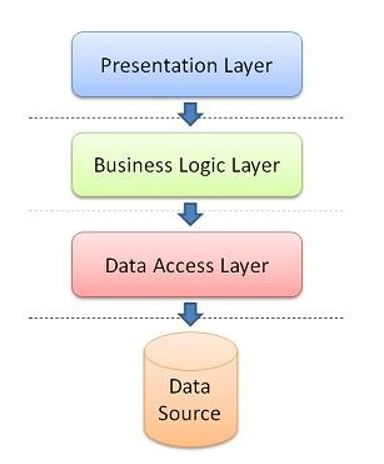
\includegraphics[scale=1]{immagini/layered_architecture}
	\caption{Schema architettura Layered 3-tier}
\end{figure}
L'architettura \textit{Layered 3-tier} è un architettura software molto semplice in cui le varie funzionalità sono separate logicamente ovvero suddivise su livelli logici differenti in comunicazione tra di loro.\\
I componenti all'interno di un'architettura di questo tipo sono organizzati in livelli orizzontali, ognuno dei quali si occupa di uno specifico ruolo all'interno del sistema completo.\\
Il pattern di questa tipologia di architettura non specifica il numero di livelli ma, nella versione più comune, il numero di livelli è tre suddiviso in: \textit{Presentation Layer}, \textit{Business Logic Layer} e \textit{Data Access Layer} il quale, poi, si occuperà di accedere ai dati all'interno del \textit{Data Source}.\\
Ogni livello, come abbiamo già visto, si occupa di uno specifico ruolo all'interno del sistema completo:
\begin{itemize}
	\item \textbf{Presentation Layer} - ha lo scopo di gestire l'interazione del sistema con il mondo esterno, in particolare con gli utenti. Include le maschere per visualizzare e inserire dati, controlli, dai più semplici ai più complessi, e i meccanismi per intercettare e gestire opportunamente tutti gli eventi che sono scatenati dalle azioni degli utenti;
	\item \textbf{Business Logic Layer} - include l'insieme delle regole di business che regolano il funzionamento dell'applicazione, intercetta le richieste provenienti dallo strato di presentazione e le gestisce opportunamente;
	\item \textbf{Data Access Layer} - conosce le modalità per leggere e salvare le informazioni interne al sistema nell'ambito di una sorgente dati (non necessariamente un database centralizzato).
\end{itemize}
\subsection{Analisi e rating dell'architettura scelta}
La seguente tabella contiene una valutazione delle principali caratteristiche dell'architettura scelta.\\
Andremo ora a spiegarle e ad analizzarle.
\begin{figure}[h]
	\centering
	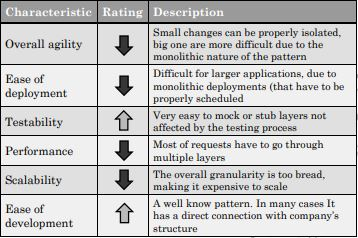
\includegraphics[scale=1]{immagini/layered_architecture_analysis}
	\caption{Analisi dell'architettura Layered 3-tier}
\end{figure}
\begin{itemize}
	\item \textbf{Overall agility}:
	\begin{itemize}
		\item \textbf{Rating}: Basso;
		\item \textbf{Analisi}: è la capacità del sistema di reagire velocemente ad un ambiente in costante cambiamento. Nonostante le modifiche siano essere isolate attraverso i livelli è comunque difficile apportare dei cambiamenti a causa della sua struttura monolitica della maggior parte delle implementazioni che lo adottano e dello stretto accoppiamento che si ha tra i livelli\cite{3tierArch}\cite{3tierArch2}.
		\item \textbf{Valutazione}: nonostante la non semplice gestione dei cambiamenti questo non è un problema per lo sviluppo del modulo \gls{ITF} in quanto, essendo il sistema sviluppato interamente appoggiandosi ad \textit{Ethereum}, le modifiche sono difficili di per sé a causa dell'immutabilità garantita ai contratti una volta che questi sono rilasciati nella rete.\\
		Per andare a modificare un contratto, l'unico modo è riscriverlo con tutte le modifiche necessarie e sostituire gli indirizzi nei contratti che lo utilizzano.\\
		Potrebbe risultare un procedimento complesso ma così non è se si adottano strategie che prevedono questo scenario (metodi di \textit{setting} degli indirizzi bloccati ai soli proprietari dei contrati).\\
	\end{itemize}
	Per questa motivazione nonostante il rating basso di questa caratteristica, il sistema non ne viene influenzato in modo negativo.
	\item \textbf{Ease of deployment}:
	\begin{itemize}
		\item \textbf{Rating}: Basso;
		\item \textbf{Analisi}: un piccolo cambiamento ad una componente può richiedere la ri-implementazione dell'intera applicazione o di una grossa porzione di essa, facendo sì che sia necessaria la pianificazione e l'implementazione durante ore non lavorative\cite{3tierArch}\cite{3tierArch2}.
		\item \textbf{Valutazione}: come per l'\textit{Overall agility} questa caratteristica non è un problema per l'implementazione del modulo se viene pensato per essere estesto in quanto, come detto nel punto precedente, essento tutto appoggiato sopra la rete \textit{Ethereum} l'implementazione di nuovi contratti o la loro modifica necessità la creazione del contratto e la sostituzione degli indirizzi all'interno dei contratti che lo utilizzano.
	\end{itemize}
	\item \textbf{Testability}:
	\begin{itemize}
		\item \textbf{Rating}: Alto;
		\item \textbf{Analisi}: siccome i componenti sono suddivisi in livelli separati è possibile creare dei mockup o degli \emph{\gls{stub}}\glsfirstoccur per i livelli che dipendono direttamente da quello che si sta sviluppando. Questo fa sì che la testabilità del sistema sia molto facile\cite{3tierArch}\cite{3tierArch2}.\\
		\item \textbf{Valutazione}: essendo, la maggior parte del modulo, appoggiato ad \textit{Ethereum} ed essendo i contratti immutabili, una volta rilasciati nella rete, si ha la necessità di operare un gran numero di test prima del rilascio in modo da evitare di dover creare un nuovo contratto che va a sostituire quello contenente errori.\\
		Per questo motivo questa caratteristica è di fondamentale importanza per il modulo \gls{ITF}.		
	\end{itemize}
	Questa caratteristica è fondamentale per l'\gls{ITF} \textit{Ethereum} e il suo rating alto è stato uno dei motivi di scelta dell'intera architettura.
	\item \textbf{Performance}:
	\begin{itemize}
		\item \textbf{Rating}: Basso
		\item \textbf{Analisi}: il pattern architetturale non si presta bene nell'avere alte performance questo è dato dal fatto che ogni volta che si vuole interagire con un livello bisogna necessariamente passare attraverso multipli livello per andare a soddisfare la richiesta\cite{3tierArch}\cite{3tierArch2}.
		\item \textbf{Valutazione}: il fatto di dover passare attraverso molti livelli senza dare la possibilità di "scavalcarne" alcuni per determinate richieste è un concetto chiave dell'architettura detto T\textit{he layers of Isolation}. Questo fa sì che ogni cambiamento ad un livello non abbia effetto su altri componenti di altri livelli: il cambiamento è isolato ai componenti interni al livello.\\
		Se si permettesse ad alcuni componenti di "scavalcare" i livelli direttamente sottostanti, i cambiamenti a questo livello influenzerebbero pesantemente tutti gli altri andando a creare un forte accoppiamento tra le parti.\\
		La considerazione da fare è che, il sistema che vogliamo realizzare, è semplice e non prevede una profondità dei livelli così alta da andare a inficiare pesantemente sulle prestazioni del modulo in più c'è da dire che la \textit{Blockchain Ethereum} è il vero freno sulle prestazioni del sistema in quanto, una transazione, potrebbe richiedere anche svariati minuti.
	\end{itemize}
	\item \textbf{Scalability}:
	\begin{itemize}
		\item \textbf{Rating}: Basso
		\item \textbf{Analisi}: la Scalabilità (capacità di un sistema di reagire a richieste di lavoro più pesanti) è un problema per i sistemi sviluppati tramite l'utilizzo di questa architettura. In un'architettura di questo tipo la scalabilità può essere ottenuta andando a dividere i vari livelli in implementazioni fisicamente separate o andando a replicare l'interna applicazione in nodi multipli\cite{3tierArch}\cite{3tierArch2}.
		\item \textbf{Valutazione}: questa caratteristica potrebbe essere l'unica in grado di andare ad intaccare il modulo \gls{ITF} se non pensato correttamente.\\
		Secondo me, il problema principale all'interno della rete \textit{Ethereum} alla quale ci andiamo ad appoggiare, è principalmente dovuto alla scrittura dei dati e quindi durante la fase di registrazione di un nuovo utente o l'aggiornamento dei certificati conseguiti.\\
		Queste essendo operazioni che avvengono con bassa frequenza (un utente si registra una sola volta in quanto l'identità digitale è unica ma condivisa per ogni servizio e l'inserimento di nuove certificazioni non è un'operazione che viene fatta ) potrebbero non avere effetti negativi nel sistema in quanto, quello che viene fatto principalmente, sono letture di dati da parte dei vari Service Providers prima di permettere il rilascio di un servizio.
	\end{itemize}
	\item \textbf{Ease of development}:
	\begin{itemize}
		\item \textbf{Rating}: Alto
		\item \textbf{Analisi}: l'Ease of development (facilità di sviluppo) raggiunge livelli molto alti soprattutto data dal fatto che è un'architettura molto semplice e conosciuta.\\
		Siccome molte compagnie ed aziende sviluppano applicazioni e sistemi andando a separare i livelli per competenze, questo pattern diventa una delle scelte migliori\cite{3tierArch}\cite{3tierArch2}.
		\item \textbf{Valutazione}: la facilità di sviluppo di un sistema basato su questa architettura è, sicuramente, una caratteristica importante.\\
		Questo viene dal fatto che, grazie ad un'architettura del genere, è possibile andare a mettere le mani nel codice in tempi molto più brevi rispetto a quelli richiesti se venisse adotta un'altra tipologia di architettura.\\
		In più, il fatto di poter dividere i vari livelli per competenze permette lo sviluppo separato e parallelo di componenti diverse senza la necessità che il sistema segua un filo logico inizio – fine.\\
		Quest'ultimo accorgimento è di fondamentale importanza in quanto è stato necessario suddividere la parte fornt-end dal back-end e lo sviluppo è avvenuto in parallelo.
	\end{itemize}
\end{itemize}
\section{Approccio alla progettazione}
Per la progettazione del modulo si è deciso di utilizzare un approccio \emph{\gls{topDown}}\glsfirstoccur. Essa consiste nel descrivere il sistema partendo da una visione generale ad alto livello per poi scendere nel particolare delle parti individuate.\\
Nella visione ad alto livello è possibile notare che il sistema è composto da diversi packages che interagiscono tra di loro. Entrando nel dettaglio si vanno ad individuare tutte le componenti più piccole e semplici tramite la strategia \textit{divide-et-impera}. L'approccio \gls{topDown} parte dall’obiettivo e da esso valorizza il "perché" e fa dipendere il "come", permettendo di suddividere il lavoro rendendolo più comprensibile e, quindi, di più facile manutenibilità.
\section{Architettura generale}
Il modulo \gls{ITF} è formato da due parti distinte:
\begin{itemize}
	\item \textbf{Front-end}:l'applicativo tramite la quale gli utenti e gli attori esterni possono interagire con l'intero sistema;
	\item \textbf{Back-end}: tutte le componenti che contengono la \textit{Business Logic}, gestiscono la presistenza dei dati interni alla \textit{Blockchain Ethereum} e le componenti necessarie a far sì che il \textit{front-end} riesca ad interagire con la \textit{Business Logic}.
\end{itemize}
Il lato \textit{back-end} prevede l'utilizzo della \textit{Blockchain Ethereum} per la gestione e la certificazione delle informazioni personali dell'utente insieme alla verifica delle informazioni da parte di un Service Provider che ha ricevuto una richiesta di accesso da parte di un utente.\\
Tutte queste operazioni vengono gestite tramite \textit{smart contracts Solidity} in modo da permettere l'interazione con l'\gls{evm}.\\
Tutte le componenti della parte \textit{back-end} sono raggruppate in packages. Questo viene fatto perchè, all'interno di ogni package, troviamo:
\begin{itemize}
	\item Gli \textit{smart contracts} che contengono i dati da gestire e dei metodi fittizi che contengono gli indirizzi ai metodi veri e propri;
	\item Gli \textit{smart contracts} contenenti l'implementazione vera e propra dei vari metodi.
\end{itemize}
Questo è necessario in quanto un contratto \textit{Ethereum}, una volta rilasciato nella rete, diventa immutabile e quindi non più modificabile in caso di malfunzionamenti o risultati inaspettati.\\
Separando la parte logica (metodi) dalla componente dati (con metodi fittizi) e collegando le due parti tramite indirizzi fa sì che l'eventuale presenza di errori possa essere gestita andando a implementare nuovamente solo la parte logica e cambiando gli indirizzi nella componente dati (questo cambiamento deve essere gestito tramite appositi metodi \textit{setter}).
\section{Componenti del modulo}
\subsection{Visione generale}
\begin{figure}[!h]
	\centering
	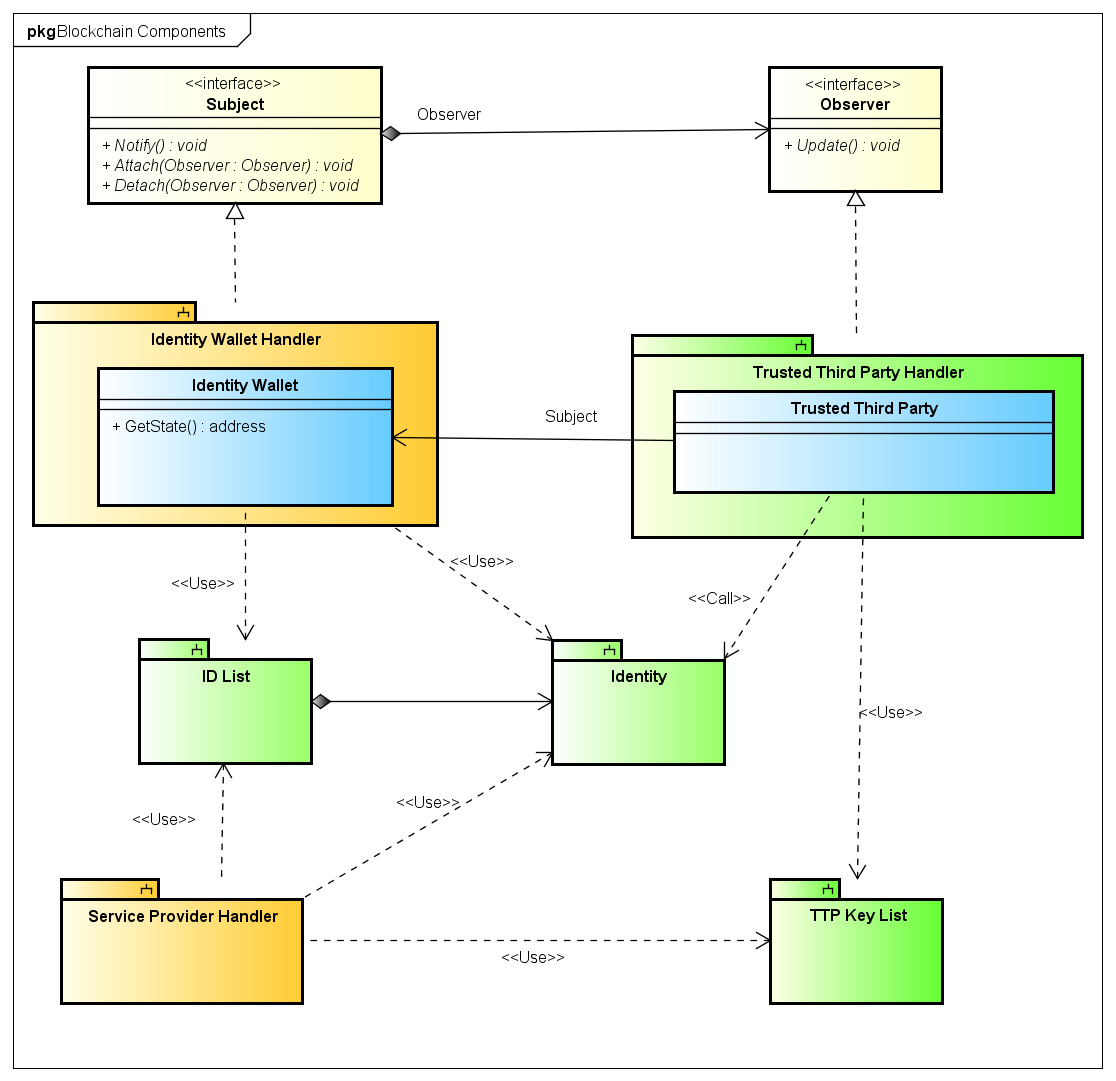
\includegraphics[width=0.5\textwidth]{immagini/architettura_alto_livello}
	\caption{Visione ad alto livello}
	\label{fig:visioneAltoLivello}
\end{figure}
\begin{itemize}
	\item \textbf{Descrizione}:\\
	Questo è il package principale dell'applicazione lato \textit{back-end}.\\
	Tutte le classi e i sottosistemi presenti in questo package contengono la \textit{business logic} e la persistenza dei dati necessari per realizzare il modulo \gls{ITF} e la sua interazione con il mondo esterno verso il Service Provider e l'Identity Wallet.
	\item \textbf{Package contenuti}:\\
	\begin{itemize}
		\item Identity Wallet Handler;
		\item ID List;
		\item Identity;
		\item TTP Key List;
		\item Trusted Third Party;
		\item Service Provider Handler.
	\end{itemize}	
\end{itemize}
Come si può vedere dallo schema in figura \ref{fig:visioneAltoLivello} le varie componenti presentano dei colori diversi. Questo è stato fatto per rendere più chiara la suddivisione dei package in base al \textit{design pattern} ad essi associati.\\
\begin{itemize}
	\item \textbf{Design pattern Observer} - formano questo design pattern: il package Identity Wallet Handler, la classe Trusted Third Party e le interfacce Subject e Observer (colore: azzurro);
	\item \textbf{Design pattern Façade} - formano questo design pattern i due package Service Provider Handler e Identity Wallet Handler (colore: arancione);
	\item \textbf{Desing pattern Strategy} - tutti i package nello schema presentano questo design pattern al loro interno quindi: Identity Wallet Handler, Service Provider Handler, ID List e Identity (colore verde).
\end{itemize}
Alcuni package non rispettano i colori sopracitati in quanto realizzano più di un design pattern. Vedremo in seguito quali.